% TEX compiler = luatex
% copyright arturo salinas-aguayo 2025
\documentclass[12pt]{article}

\usepackage{graphicx}
\usepackage{amsmath}
\usepackage{array}
\usepackage{amsfonts}
\usepackage{fancyhdr}
\usepackage{geometry}
\usepackage{subfigure}
\usepackage{caption}
\usepackage{karnaugh-map}
\usepackage{bm}
\usepackage{float}

\geometry{letterpaper, margin=1in}
\graphicspath{ {../../images/} }

% Header and Footer
\pagestyle{fancy}
\fancyhf{}
\fancyhead[L]{ECE 2001 - Design Project 1: A Music and Microphone Mixer}
\fancyhead[R]{\thepage}
\setlength{\headheight}{15pt}

\author{Arturo Salinas-Aguayo}
\title{Design Project 1: A Music and Microphone Mixer}
% theorem set
\newtheorem{example}{Example}
% Example block environment
\newenvironment{examp}
{\vspace{0.5cm}
 \hrule
\vspace{0.5cm}
\begin{example}}
{\hrule
\vspace{0.5cm}
\end{example}}

\begin{document}
\newcommand{\closure}[2][3]{%
	{}\mkern#1mu\overline{\mkern-#1mu#2}}
\newcommand\ncoverline[1]{\mkern1mu\overline{\mkern-1mu#1\mkern-1mu}\mkern1mu}
% Title Page
\begin{titlepage}
	\centering
	\vspace*{3cm}
	\huge\textbf{Design Project 1: A Music and Microphone Mixer}\\
	\vspace{5cm}
	\Large\textbf{Arturo Salinas-Aguayo}\\
	\normalsize
	ECE 2001 Electrical Circuits\\
	Dr. David J. Giblin, Section 331.660.701.810-1253\\
	Mechanical Engineering Department
	\vfill
	
\includegraphics[scale=0.1]{uconnlogo}\\
	College of Engineering, University of Connecticut\\
	\scriptsize{Coded in \LaTeX}
	\vspace*{1cm}
\end{titlepage}
\tableofcontents
\newpage
\section{Abstract}
For the first design project of this course, the theory learned in the past
experiment utilizing basic operation amplifiers and driving an $8\Omega$ speaker
is built upon. Audio signals come in many different shapes depending on the
excitation source, and by utilizing two very different sources, a 1.5mm Line Out
from a computer and a electret microphone, the challenges of designing a circuit
which can amplify both of these signals to target specification becomes
apparent.

Audio applications of analog circuits are amongst the most
popular for this subset of circuitry that is being studied. That being said,
being able to handle a modulating wave of various amplitudes and designing a
circuit which can handle two audio signals that can be independantly mixed is a
neat challenge in elementary circuit design. The operational amplifier can be
used in different ways such as an inverting or a summing amplifier, and in
conjunction with potentiometers, can be utilized to create a simple circuit
which can achieve this very purpose. Opamps make life a great deal easier for
the audio circuit builder and knowing the characteristics of each of these
different building blocks allows for a wide variety of implementations.
\newpage
\section{Introduction}
The practical operation of Opamps is quite straightforward, it takes a signal
and depending on the configuration, the output is simply a greatly amplified
version of the difference between the two signals. The task at hand is to
amplify two different signals from two discrete inputs according to
specification to achieve operation similar to a music mixer. Two potentiometers
operate as the volume knobs adjusting the gain of the signals to change the
characteristics of the circuit in real time, allowing for the proper
amplification of the signals.

The first signal is from the Line Out of a computer acting as a music input
which has a strong peak to peak voltage reading of $1.5V$. The second input is
from a much weaker electret condenser microphone which outputs a peak to peak
voltage of $1.5mV$.

The star of this particular experiment is once again the $\mu A741$ which as
stated in previous experiments, is quite an older design of the operational
amplifier which is not optimal for audio amplification purposes, however for
learning purposes it does just fine. With an input voltage differential of
$10V$ for the experiment, cascading is utilized in order to prevent saturation
of the audio signals at each stage.

The target output is the $8\Omega$ speaker used previously as well. Designing to
a target specification of $275mW$ peak power, this provides a way to design each
of the cascading operational amplification stages to achieve.

The use of noise filtering components such as capacitors and other more common
devices is restricted to a single input capacitor for each input which changes
the frequency response characteristics of the circuit quite minimally. Once the
circuit is designed and implemented, the frequency and phase response of each
input is measured against each input with the opposite input grounded out to
minimize noise. Signal-to-Noise ratios are an important characteristic when
designing these circuits, and significantly designing for the total circuit
environment must be considered to minimize noise and maximize the dynamic range
and signal fidelity of the circuit design.

To measure and apply the reference signals, Scopy is used in conjunction with
the ADALM2000 once again. This brings its own challenge as the sensitivity of
the instrument struggles to obtain a clean waveform of such a small amplitude
when simulating the microphone input, however the circuit design and operational
characteristics hold true and allowed for a somewhat noisy signal to be recorded
and plotted alongside the simulation.
\section{Theory}
To begin with the design, careful consideration to how much gain from each input
must be first calculated.
\subsection{Target Gains}
The specifications were given to design a circuit that can amplify a $1.5V$ and
a $3mV$ peak-to-peak signal to $275mW$ peak power. Engineers must be able to
decode these design specifications and understand what they actually mean. A
peak signal refers to the amplitude of a waveform, while a peak-to-peak
measurement refers to the top crest of the wave measured against the bottom
crest, or double the amplitude of the waveform.


Starting with the output, a $275mW$ peak power with a resistance of $8\Omega$ produces the following equation according to Ohm's Law (see Experiment 1):
\begin{equation}
	P = \frac{V_{rms}^2}{R}
\end{equation}
where $P$ is the power, $V_{rms}$ is the root mean square voltage, and $R$ is the resistance. Substituting the given values:
\begin{equation}
	0.275W = \frac{V_{rms}^2}{8\Omega}
\end{equation}
Solving for $V_{rms}$:
\begin{equation}
	V_{rms} = \sqrt{0.275W \times 8\Omega} = \sqrt{2.2} \approx 1.48V
\end{equation}
Since peak voltage $V_p$ is related to $V_{rms}$ by $V_p = \sqrt{2} V_{rms}$:
\begin{equation}
	V_p = \sqrt{2} \times 1.48V \approx 2.0V
\end{equation}
Thus, the design peak voltage specification is approximately $2.0V$, and the peak-to-peak voltage is:
\begin{equation}
	V_{pp} = 2 \times V_p = 4.0V
\end{equation}
\subsection{Total Gain Calculation}

To determine the required gain, we compare the input peak-to-peak voltages with the required output peak voltage of $2V$.

For the $1.5V$ peak-to-peak signal:
\begin{equation}
	V_{in} = \frac{1.5V}{2} = 0.75V \text{ (peak)}
\end{equation}
The required voltage gain is:
\begin{equation}
	A_v = \frac{V_{out}}{V_{in}} = \frac{2V}{0.75V} = 2.67
\end{equation}

For the $3mV$ peak-to-peak signal:
\begin{equation}
	V_{in} = \frac{3mV}{2} = 1.5mV \text{ (peak)}
\end{equation}
The required voltage gain is:
\begin{equation}
	A_v = \frac{V_{out}}{V_{in}} = \frac{2V}{1.5mV} = 1333.33
\end{equation}

Thus, the circuit must provide a voltage gain of approximately $2.67$ for the $1.5V$ input signal and $1333.33$ for the $3mV$ input signal.

\subsection{Cascading Operational Amplifiers}

Now that the target gains for each half of the circuit are known, the next step
is to implement a circuit capable of achieving these gains without saturating at
a single stage. Additionally, the circuit must allow adjustable control via a
$10k\Omega$ potentiometer.

To accomplish this, the following building blocks were considered:

\subsubsection{The Inverting Amplifier}

This configuration, also known as a \textit{Voltage Shunt Feedback Amplifier},
is one of the simplest and most commonly used configurations. The overall gain
of this stage depends solely on the ratio of the resistors $R_f$ and $R_1$, as
shown in Figure \ref{fig:invertingamp}.

\begin{figure}[H] \centering 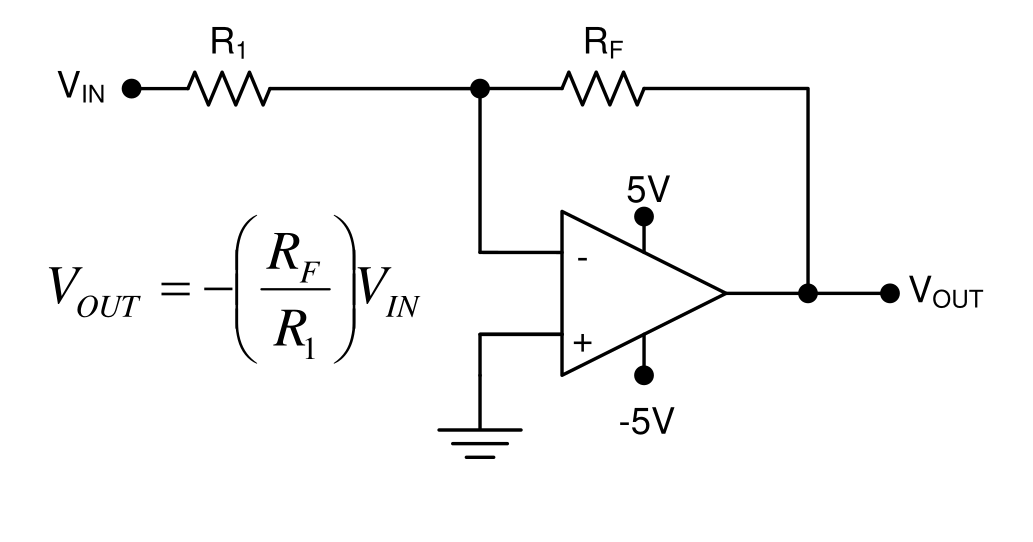
\includegraphics[width=8cm]{dp_02} \caption{The
		Inverting Amplifier} \label{fig:invertingamp} \end{figure}

Using principles discussed in previous experiments, such as the virtual ground
and input impedance: \begin{equation} A_f = - \frac{R_f}{R_1} \end{equation}

The negative sign indicates that the output voltage is $180^\circ$ out of phase
with the input signal voltage. However, for audio amplification purposes, the
phase shift is imperceptible to the human ear, unless signals need to be mixed
into a unified waveform, which is not a requirement in this design.

By selecting appropriate values for $R_f$ and $R_1$, the gain can be adjusted to
the desired value. If $R_f$ is a short circuit (0$\Omega$), the gain is
effectively zero. This property allows the use of a $10k\Omega$ potentiometer as
$R_f$, enabling variable gain control.

\subsubsection{The Summing Amplifier}

The \textit{summing} function of an operational amplifier allows multiple input
voltages to be summed at the negative terminal. As an extension of the Inverting
Amplifier, it operates similarly but accepts multiple inputs at the input node,
as shown in Figure \ref{fig:summingamp}.

\begin{figure}[H] \centering 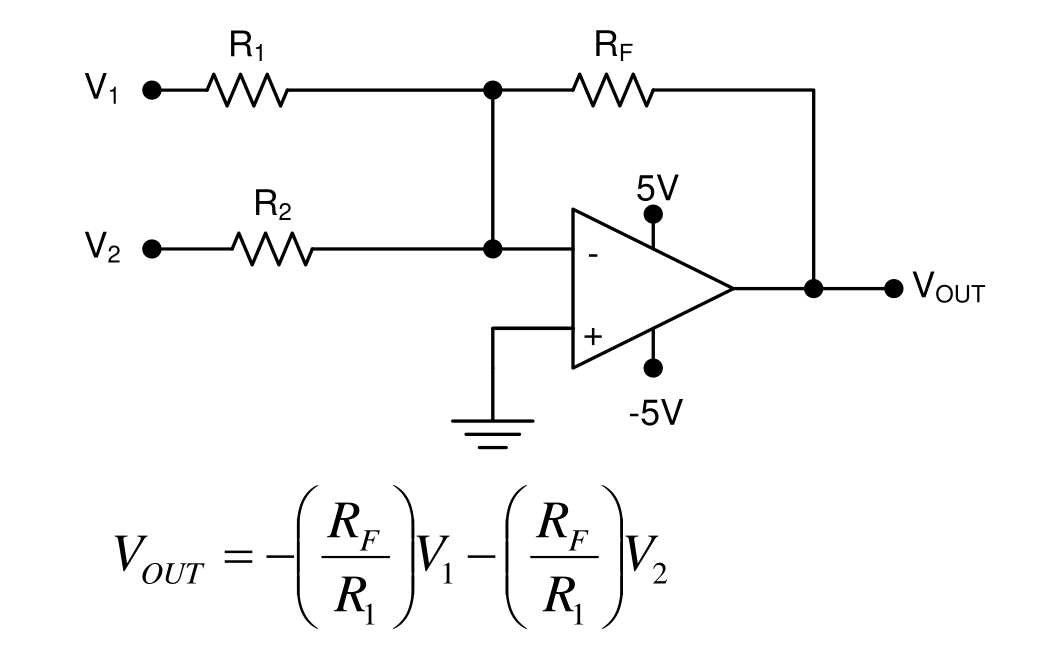
\includegraphics[width=8cm]{dp_01} \caption{The
		Summing Amplifier} \label{fig:summingamp} \end{figure}

By selecting appropriate resistor values, a target gain can be achieved based on
the input and output relationship: \begin{equation} V_{out} = -\left(
	\frac{R_f}{R_1}V_1 + \frac{R_f}{R_2}V_2 \right) \end{equation}

Again, the negative sign results from the inverting nature of the configuration.

\subsubsection{Combining Stages}

When cascading these amplification stages, the overall gain of the system is the
product of the individual stage gains. This progressive approach allows the
circuit to reach the desired gain while maintaining stability and preventing
over-saturation in a single stage.

The final design incorporates the Inverting Amplifier and Summing Amplifier,
along with a Push-Pull amplifier to provide a continuous current source for
driving the output speaker, as previously discussed in Experiment 4.

\subsection{Decibel Gain Calculation}

In frequency response analyses, gains are expressed in decibels (dB) for convenience, clarity, and ease of interpretation. The decibel scale is logarithmic, reflecting how humans perceive changes in loudness. The voltage gain ($A_v$) in decibels is calculated using the formula:

\begin{equation}
	A_v(\text{dB}) = 20 \cdot \log_{10}\left(\frac{V_{\text{out}}}{V_{\text{in}}}\right)
\end{equation}

Here:
\begin{itemize}
	\item $V_{\text{out}}$ is the measured output voltage amplitude.
	\item $V_{\text{in}}$ is the measured input voltage amplitude.
\end{itemize}

A gain increase of $6\,dB$ corresponds approximately to doubling the voltage amplitude, and a $-3\,dB$ point indicates the frequency at which the output power has dropped to half of its maximum amplitude power (approximately 70.7\% of maximum voltage amplitude).

\subsection{The Final Design}
To achieve the design specifications, two inverting amplifier stages, followed by a final summing amplifier stage, were employed for each input signal. This approach was essential to account for the vastly different amplitudes of the two input signals. The circuit design utilized cascading amplifier stages to progressively amplify each signal without overloading any single stage. This method ensures that each amplifier operates within its optimal range while still achieving the necessary overall gain. The resulting circuit configuration is shown in Figure \ref{fig:fullcircuit}.

\begin{figure}[H]
	\centering
	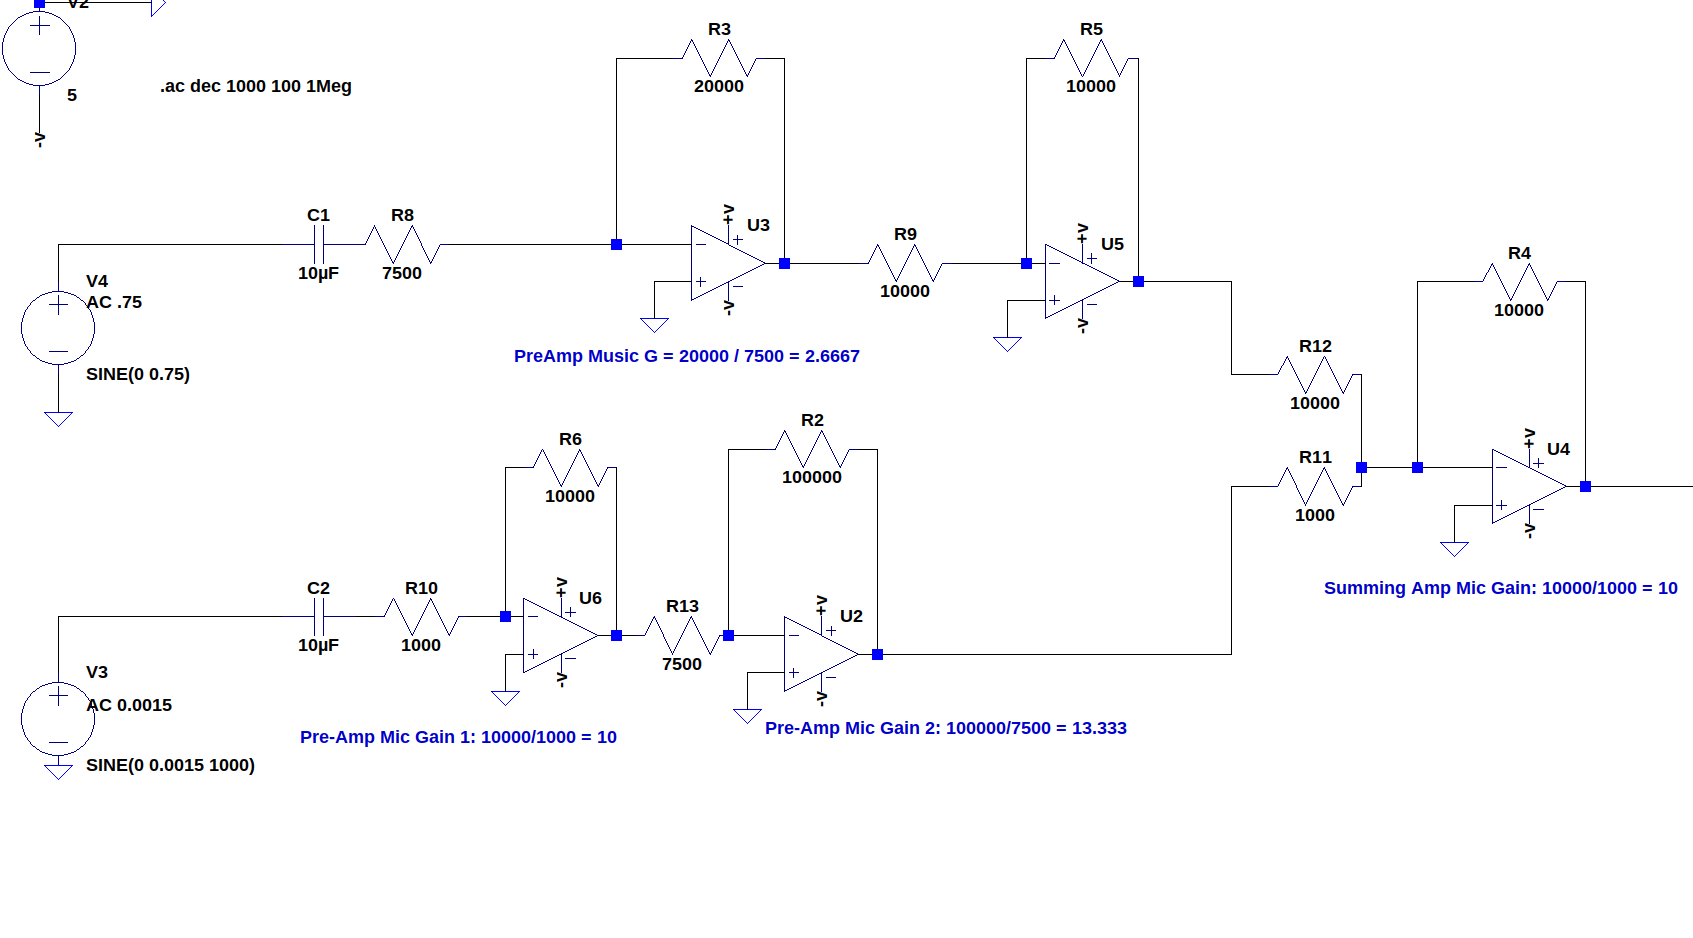
\includegraphics[width=1\textwidth]{dp_03}
	\caption{The Final Cascaded Design}
	\label{fig:fullcircuit}
\end{figure}

\subsubsection{The Music Input}
For the music input, the first stage is a static inverting amplifier with a fixed gain of $2.667$. This gain is realized using standard resistors available in the experimentation kit. The values for the resistors $R_f$ and $R_1$ were chosen as follows to achieve the desired gain:

\begin{align*}
	R_f = R_3 = 20000\Omega, \quad & \quad R_1 = R_8 = 7500\Omega \\
	\text{Gain} = \frac{R_f}{R_1} = \frac{20000}{7500} = 2.6667
\end{align*}

The output of this first stage is then fed into a second stage, which uses a potentiometer as the feedback resistor. The potentiometer provides variable control over the gain, allowing the audio gain to be adjusted in real time from $0$ to the target power of $275mW$. This stage has a maximum gain of $1$, ensuring that the amplification process remains linear and the final signal can be fine-tuned as needed. The resistors in this stage were chosen to allow for this linearity:

\begin{align*}
	R_f = R_5 = 10000\Omega, \quad & \quad R_1 = R_9 = 10000\Omega \\
	\text{Gain} = 1
\end{align*}

The final stage for the music input is the summing amplifier, which is configured similarly with no additional gain. The summing amplifier mixes the input signals while maintaining the original gain factor of $1$ for each input:

\begin{align*}
	R_f = R_4 = 10000\Omega, \quad & \quad R_1 = R_{12} = 10000\Omega \\
	\text{Gain} = 1
\end{align*}

Thus, the total gain for the music input is:

\begin{equation}
	\text{Total Gain} = 2.6667 \cdot 1 \cdot 1 = 2.6667
\end{equation}

This gain factor is consistent with the requirements for amplifying the music input signal to the desired level.

\subsubsection{The Microphone Input}
For the microphone input, special care had to be taken with each amplification stage to prevent oversaturation of the operational amplifiers. Since the microphone signal has a much lower amplitude compared to the music input, each stage needed to provide more substantial amplification. The first stage, using a potentiometer, acts as the initial amplifier. The potentiometer is constrained to a $10k\Omega$ resistance, and the first stage resistor must also be chosen carefully to avoid excessive noise. In this case, a $1k\Omega$ resistor was used for the first stage, setting the tone for the subsequent stages.

The gain for this first stage is calculated as follows:

\begin{align*}
	R_f = R_6 = 10000\Omega, \quad & \quad R_1 = R_{10} = 1000\Omega \\
	\text{Gain} = \frac{R_f}{R_1} = \frac{10000}{1000} = 10
\end{align*}

After the initial amplification, the second stage is designed to provide a larger gain. Given the low amplitude of the microphone signal, this stage amplifies the signal further to reach the desired output. The resistor values are chosen to ensure sufficient amplification while keeping the system stable:

\begin{align*}
	R_f = R_2 = 1000000\Omega, \quad & \quad R_1 = R_{13} = 7500\Omega \\
	\text{Gain} = \frac{R_f}{R_1} = \frac{1000000}{7500} = 1333.33
\end{align*}

The final stage for the microphone input is the summing amplifier, which is used to mix the signals from both stages and achieve the final desired output. The gain factor for this stage is calculated as follows to bring the total gain for the microphone input to the required value:

\begin{align*}
	R_f = R_4 = 10000\Omega, \quad & \quad R_1 = R_{11} = 1000\Omega \\
	\text{Gain} = \frac{R_f}{R_1} = \frac{10000}{1000} = 10
\end{align*}

Thus, the total gain for the microphone input is:

\begin{equation}
	\text{Total Gain} = 10 \cdot 13.3333 \cdot 10 = 1333.333
\end{equation}

This high gain factor ensures that the microphone signal, initially weak and requiring substantial amplification, is amplified to the required level suitable for output through the speaker.

\section{Experimental Procedures}
Prior to conducting any experimental measurements, the designed mixer circuit was thoroughly analyzed using simulation software (LTSpice). This preliminary simulation step is essential, as it validates the theoretical design, identifies potential issues, and provides baseline data for subsequent experimental validation.

\subsection{PSpice (LTSpice) Simulation Setup}

The frequency response characteristics were determined by performing an AC sweep analysis on the mixer circuit (excluding the power amplifier and speaker stage). The following steps outline the simulation procedure clearly:

\begin{enumerate}
	\item \textbf{Circuit Configuration:}
	      \begin{itemize}
		      \item The mixer circuit was modeled precisely according to the schematic, excluding the final amplification stage (speaker output).
		      \item For music channel characterization, the microphone input was
		            grounded, and a sinusoidal AC voltage source (VAC) was applied to
		            the music input with an amplitude of $0.75\,V$.
		      \item For microphone channel characterization, the music input was
		            grounded, and the microphone input was supplied with a sinusoidal
		            VAC of $1.5\,mV$ amplitude.
	      \end{itemize}
	      
	\item \textbf{AC Sweep Simulation:}
	      \begin{itemize}
		      \item The frequency sweep spanned from $100\,Hz$ to $1\,MHz$, with at least 100 logarithmically spaced frequency points.
		      \item Voltage markers were placed at both input and output nodes to measure amplitude response, calculated using the formula:
		            \[
			            \text{Gain (dB)} = 20 \cdot \log_{10}\left(\frac{V_{\text{out}}}{V_{\text{in}}}\right)
		            \]
		      \item Phase response was obtained by placing a phase probe at the output node of the circuit.
		      \item Data from LTSpice simulations was exported for subsequent comparison with experimental results.
	      \end{itemize}
\end{enumerate}

\subsection{Experimental Measurements}

The experimental verification involved constructing the mixer circuit on a breadboard, ensuring accurate wiring and proper component selection. The following steps detail the measurement procedure:

\begin{enumerate}
	\item \textbf{Gain Verification at 2 kHz:}
	      \begin{itemize}
		      \item A $2\,kHz$ sinusoidal input was applied separately to each channel.
		      \item The maximum and minimum adjustable gains were verified for both music and microphone channels using a potentiometer to adjust the amplitude.
		      \item Gain was calculated experimentally by measuring the input and
		            output voltages on Scopy and employing the decibel conversion
		            mentioned above.\\
		            
		            LTSpice Gain at 2 kHz: \textbf{8.78 dB}\\
		            Scopy Gain at 2 kHz: \textbf{8.19 dB}\\
		            LTSpice Gain at 2 kHz (Mic): \textbf{20.23 dB}\\
		            Scopy Gain at 2 kHz (Mic): \textbf{20.09 dB}\\
	      \end{itemize}
	      
	\item \textbf{Frequency Response Measurements:}
	      \begin{itemize}
		      \item Frequency response was measured independently for both music and microphone channels, with the alternate input grounded to avoid cross-channel interference.
		      \item Input signals were sinusoidal, with amplitudes of $0.75\,V$ for
		            the music channel and $1.5\,mV$ for the microphone channel, as specified earlier.
		      \item Measurements were taken at approximately ten logarithmically spaced points per decade of frequency (e.g., $100\,Hz$, $200\,Hz$, $500\,Hz$, $1\,kHz$, $2\,kHz$, $5\,kHz$, etc.), spanning from $100\,Hz$ up to $1\,MHz$.
		      \item Voltage amplitude and phase measurements were recorded using the ADALM2000 instrument and the Scopy software interface.
		      \item Recorded voltage data was converted into decibels (dB) and phase shifts were noted directly from Scopy measurements.
		      \item All raw measurement data was carefully recorded and tabulated for further analysis.
	      \end{itemize}
\end{enumerate}


\section{Results and Discussion}

The experimental frequency response closely matched simulated results at lower frequencies. However, notable discrepancies and increased noise were observed at higher frequencies, especially for the microphone channel, due to its higher gain requirements.

\subsection{Noise Analysis and Observations}

During measurements, significant noise became apparent, especially for the
microphone channel at frequencies beyond $100\,kHz$. The lower amplitude of the
microphone input ($3\,mV$) necessitated substantially higher gain, amplifying intrinsic circuit noise and measurement artifacts introduced by parasitic capacitances, breadboard wiring inductances, and electromagnetic interference from lab equipment.

The noise observed in the experimental data manifests as irregular fluctuations in amplitude and phase measurements, complicating precise identification of cutoff frequencies. Nonetheless, by averaging multiple measurements and carefully interpreting the trends, reliable cutoff frequencies and general behavior were still identifiable and consistent with theoretical expectations.

\subsection{Impact of Operational Amplifier Limitations}

The $\mu A741$ operational amplifier used in the design has inherent limitations such as limited bandwidth, relatively high noise levels, and susceptibility to slew-rate distortion. These factors significantly contributed to the observed noise, especially at high frequencies where the operational amplifier struggled to maintain linear amplification, resulting in distorted waveforms and unstable measurements.

Replacing the $\mu A741$ with a modern, low-noise, higher-bandwidth operational amplifier could greatly improve the noise performance and extend the practical frequency response of the circuit.
After performing both simulated (LTSpice) and experimental (Scopy) analyses,
clear frequency response curves were generated for both the music and microphone
input channels. The AC frequency sweep ranged from $100\,Hz$ to $1\,MHz$, with
input amplitudes set at $0.75\,V$ for the music input and a larger test
amplitude of $1.5\,mV$ for the microphone input due to its significantly lower initial signal level.
\subsection{Music Channel Frequency Response}

Figure \ref{fig:music_bode} illustrates the amplitude and phase response of the music input, comparing LTSpice simulations to Scopy experimental measurements. The key findings are as follows:

\begin{figure}[H]
	\centering
	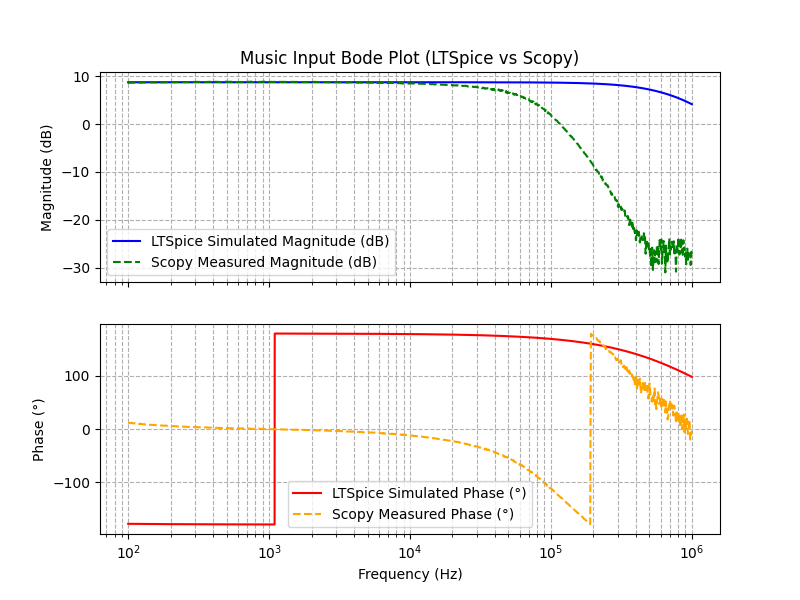
\includegraphics[width=1.0\textwidth]{dp_music}
	\caption{Music Input Bode Plot (LTSpice vs. Scopy)}
	\label{fig:music_bode}
\end{figure}

The experimentally determined upper cutoff frequency, defined as the point where
the amplitude drops by $3\,dB$ from its maximum value, was approximately
$84.344\,kHz$. The associated measured phase shift at this frequency was about
$107^\circ$. The close alignment of the experimental and simulated amplitude and phase responses validates the accuracy of the designed circuit and measurement methodology.

By Inspection,
\begin{itemize}
	\item \textbf{Cutoff Frequency:} $\approx 84.334\,kHz$
	\item \textbf{Phase Shift at Cutoff:} $\approx 107^\circ$
\end{itemize}

\begin{table}[H]
	\centering
	\footnotesize
	\caption{Music Input Data Table: Frequency Response from LTSpice and Scopy}
	\label{tab:music_data}
	\renewcommand{\arraystretch}{.9}
	\begin{tabular}{|r|r|r|r|r|}
		\hline
		\textbf{Freq (Hz)} & \textbf{LT Mag (dB)} & \textbf{SC Mag (dB)} & \textbf{LT Phase (°)} & \textbf{SC Phase (°)} \\ \hline
		100                & 8.774                & 8.828                & -178.79               & 11.70                 \\ \hline
		200                & 8.775                & 8.796                & -179.41               & 5.57                  \\ \hline
		500                & 8.776                & 8.878                & -179.81               & 1.58                  \\ \hline
		1000               & 8.776                & 8.831                & -179.98               & -0.39                 \\ \hline
		2000               & 8.776                & 8.819                & 179.86                & -2.47                 \\ \hline
		5000               & 8.776                & 8.715                & 179.52                & -6.27                 \\ \hline
		10000              & 8.775                & 8.547                & 179.00                & -12.22                \\ \hline
		20000              & 8.773                & 8.175                & 177.98                & -22.97                \\ \hline
		50000              & 8.758                & 6.633                & 174.95                & -55.18                \\ \hline
		100000             & 8.706                & 1.878                & 169.91                & -112.02               \\ \hline
	\end{tabular}
\end{table}
The amplitude response closely follows the simulation until approximately $500\,kHz$, after which discrepancies due to parasitic capacitances and real-world measurement limitations become more prominent.

\subsection{Microphone Channel Frequency Response}

Figure \ref{fig:mic_bode} shows the Bode plot for the microphone channel, again comparing LTSpice simulations and experimental Scopy measurements.

\begin{figure}[H]
	\centering
	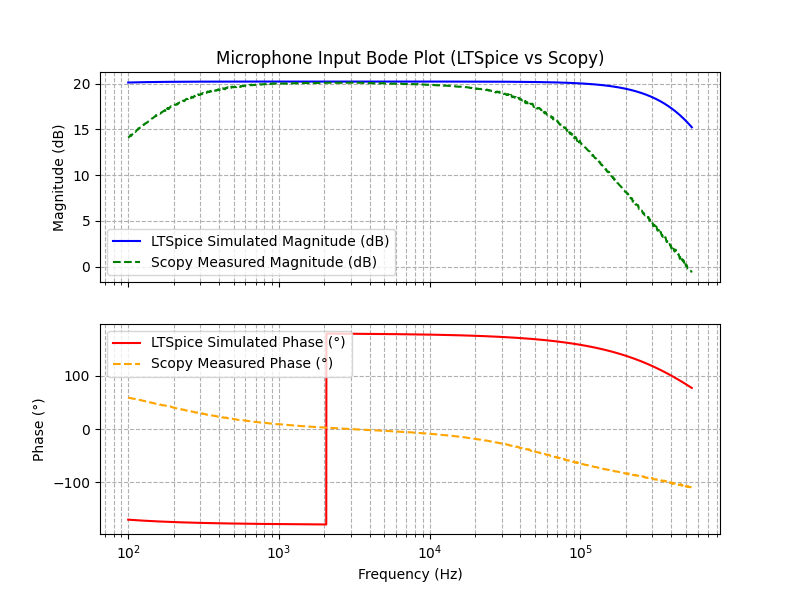
\includegraphics[width=15cm]{dp_mic}
	\caption{Microphone Input Bode Plot (LTSpice vs. Scopy)}
	\label{fig:mic_bode}
\end{figure}

For the microphone channel, the experimentally determined upper cutoff frequency
was significantly lower, observed at approximately $41.687\,kHz$. At this
frequency, a phase shift of approximately $97.933^\circ$ was recorded. This lower cutoff frequency is expected due to the significantly higher gain requirements of the microphone input stage, making it more susceptible to bandwidth limitations inherent in the $\mu A741$ operational amplifier.

By Inspection,
\begin{itemize}
	\item \textbf{Cutoff Frequency:} $\approx 41.687\,kHz$
	\item \textbf{Phase Shift at Cutoff:} $\approx 97.933^\circ$
\end{itemize}

\begin{table}[H]
	\centering
	\footnotesize
	\caption{Microphone Input Data Table: Frequency Response from LTSpice and Scopy}
	\label{tab:mic_data}
	\renewcommand{\arraystretch}{0.9}
	\begin{tabular}{|r|r|r|r|r|}
		\hline
		\textbf{Freq (Hz)} & \textbf{LT Mag (dB)} & \textbf{SC Mag (dB)} & \textbf{LT Phase (°)} & \textbf{SC Phase (°)} \\ \hline
		100                & 20.120               & 14.097               & -170.98               & 59.08                 \\ \hline
		200                & 20.201               & 17.607               & -175.49               & 40.25                 \\ \hline
		500                & 20.224               & 19.598               & -178.28               & 18.88                 \\ \hline
		1000               & 20.227               & 20.006               & -179.30               & 8.91                  \\ \hline
		2000               & 20.228               & 20.085               & -179.97               & 2.68                  \\ \hline
		5000               & 20.228               & 20.024               & 179.11                & -3.45                 \\ \hline
		10000              & 20.226               & 19.872               & 177.95                & -9.05                 \\ \hline
		20000              & 20.220               & 19.494               & 175.77                & -18.69                \\ \hline
		50000              & 20.177               & 17.545               & 169.34                & -42.55                \\ \hline
		100000             & 20.026               & 13.573               & 158.73                & -65.35                \\ \hline
	\end{tabular}
\end{table}
Experimental measurements for the microphone input exhibited more pronounced
noise and variability, primarily due to the sensitivity of the measurement
equipment at the lower input amplitude of $1.5\,mV$ and the higher total gain of the circuit. Nonetheless, the trends match closely with the simulated results, validating the overall correctness of the design.

\section{Conclusion}
The experimental results closely align with the LTSpice simulations, providing confidence in both the theoretical design and practical implementation. Minor discrepancies observed at high frequencies can be attributed to measurement noise, parasitic capacitances, and limitations inherent to the experimental setup.

It is important to note the differences between the implementation in the
protoboard compared to the simulation in LTSpice. LTSpice is simulating an ideal
Operational Amplifier which adheres strictly to the theory of the Op Amp
described in past experiments. Due to this, there is variation on the projected
phase and the generated one in Scopy.

The lower cutoff frequency of the microphone input highlights the trade-offs
involved when dealing with high-gain audio amplification, such as reduced
bandwidth and increased noise susceptibility. These practical insights underline
the importance of careful circuit layout, component selection, and supply
voltage considerations to achieve optimal audio fidelity. There is some
optimization to be had in attempting to reach such a high amplification level
for the microphone input, while still adhering to design specifications, however
due to the operational amplifier used, there are many limitations to this
practically for now.

Overall, this design project has successfully demonstrated a practical, from the
ground up design and implementation of basic operational amplifier circuitry,
with minimal need for more advanced components.

\end{document}
% vim: set ft=tex tw=80 ts=2 sts=2 sw=2 noet spell:
